% Options for packages loaded elsewhere
\PassOptionsToPackage{unicode}{hyperref}
\PassOptionsToPackage{hyphens}{url}
%
\documentclass[
]{book}
\usepackage{lmodern}
\usepackage{amsmath}
\usepackage{ifxetex,ifluatex}
\ifnum 0\ifxetex 1\fi\ifluatex 1\fi=0 % if pdftex
  \usepackage[T1]{fontenc}
  \usepackage[utf8]{inputenc}
  \usepackage{textcomp} % provide euro and other symbols
  \usepackage{amssymb}
\else % if luatex or xetex
  \usepackage{unicode-math}
  \defaultfontfeatures{Scale=MatchLowercase}
  \defaultfontfeatures[\rmfamily]{Ligatures=TeX,Scale=1}
\fi
% Use upquote if available, for straight quotes in verbatim environments
\IfFileExists{upquote.sty}{\usepackage{upquote}}{}
\IfFileExists{microtype.sty}{% use microtype if available
  \usepackage[]{microtype}
  \UseMicrotypeSet[protrusion]{basicmath} % disable protrusion for tt fonts
}{}
\makeatletter
\@ifundefined{KOMAClassName}{% if non-KOMA class
  \IfFileExists{parskip.sty}{%
    \usepackage{parskip}
  }{% else
    \setlength{\parindent}{0pt}
    \setlength{\parskip}{6pt plus 2pt minus 1pt}}
}{% if KOMA class
  \KOMAoptions{parskip=half}}
\makeatother
\usepackage{xcolor}
\IfFileExists{xurl.sty}{\usepackage{xurl}}{} % add URL line breaks if available
\IfFileExists{bookmark.sty}{\usepackage{bookmark}}{\usepackage{hyperref}}
\hypersetup{
  pdftitle={ハローワークデータからみる求人・求職活動},
  pdfauthor={川田恵介},
  hidelinks,
  pdfcreator={LaTeX via pandoc}}
\urlstyle{same} % disable monospaced font for URLs
\usepackage{longtable,booktabs}
\usepackage{calc} % for calculating minipage widths
% Correct order of tables after \paragraph or \subparagraph
\usepackage{etoolbox}
\makeatletter
\patchcmd\longtable{\par}{\if@noskipsec\mbox{}\fi\par}{}{}
\makeatother
% Allow footnotes in longtable head/foot
\IfFileExists{footnotehyper.sty}{\usepackage{footnotehyper}}{\usepackage{footnote}}
\makesavenoteenv{longtable}
\usepackage{graphicx}
\makeatletter
\def\maxwidth{\ifdim\Gin@nat@width>\linewidth\linewidth\else\Gin@nat@width\fi}
\def\maxheight{\ifdim\Gin@nat@height>\textheight\textheight\else\Gin@nat@height\fi}
\makeatother
% Scale images if necessary, so that they will not overflow the page
% margins by default, and it is still possible to overwrite the defaults
% using explicit options in \includegraphics[width, height, ...]{}
\setkeys{Gin}{width=\maxwidth,height=\maxheight,keepaspectratio}
% Set default figure placement to htbp
\makeatletter
\def\fps@figure{htbp}
\makeatother
\setlength{\emergencystretch}{3em} % prevent overfull lines
\providecommand{\tightlist}{%
  \setlength{\itemsep}{0pt}\setlength{\parskip}{0pt}}
\setcounter{secnumdepth}{5}
\usepackage{booktabs}
\ifluatex
  \usepackage{selnolig}  % disable illegal ligatures
\fi
\usepackage[]{natbib}
\bibliographystyle{apalike}

\title{ハローワークデータからみる求人・求職活動}
\author{川田恵介}
\date{2021-05-19}

\begin{document}
\maketitle

{
\setcounter{tocdepth}{1}
\tableofcontents
}
\hypertarget{ux8981ux7d04}{%
\chapter{要約}\label{ux8981ux7d04}}

公的職業紹介業務(ハローワーク)を通じて収集された業務データ(職業安定業務統計)を用いて、日本の求人・求職の状況を概観する。

\hypertarget{ux8a18ux8ff0ux7d71ux8a08ux91cf}{%
\chapter{記述統計量}\label{ux8a18ux8ff0ux7d71ux8a08ux91cf}}

\begin{itemize}
\item
  1963年から2020年までの年次データを用いて、厚生変化を記述する
\item
  就職件数の推移
\end{itemize}

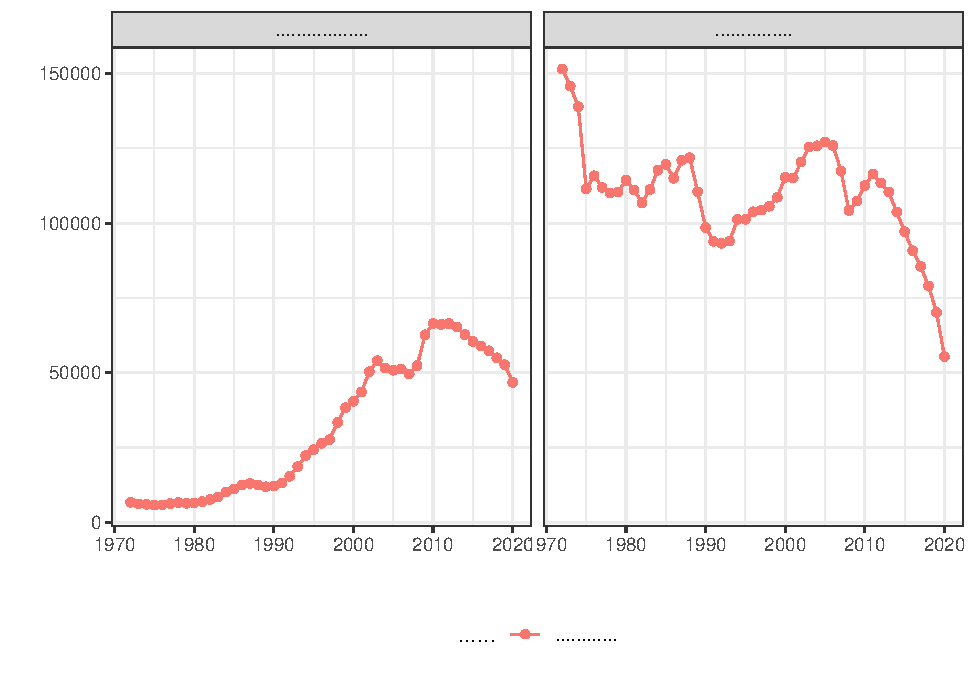
\includegraphics{test_files/figure-latex/unnamed-chunk-4-1.pdf}

\begin{itemize}
\tightlist
\item
  求人、求職件数の推移
\end{itemize}

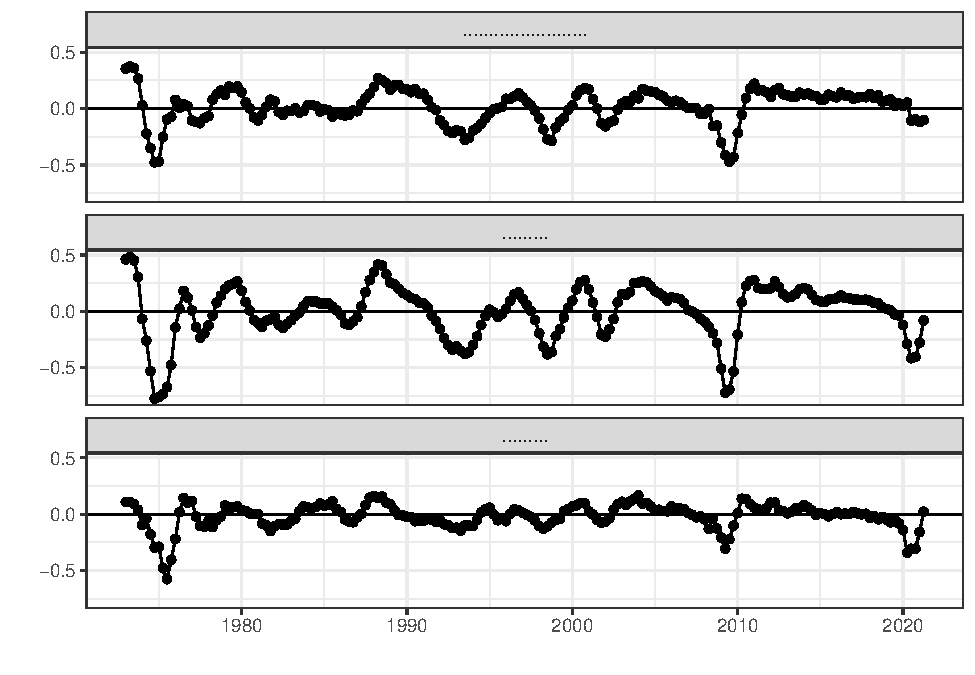
\includegraphics{test_files/figure-latex/unnamed-chunk-5-1.pdf}

\begin{itemize}
\tightlist
\item
  入職。充足率の推移
\end{itemize}

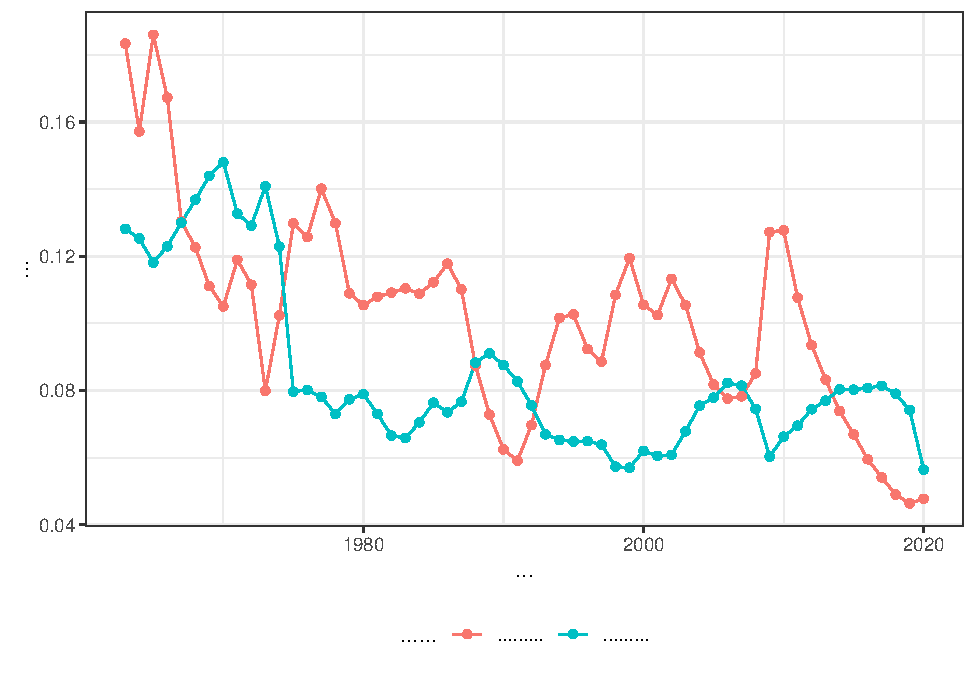
\includegraphics{test_files/figure-latex/unnamed-chunk-6-1.pdf}

\hypertarget{ux539aux751fux5206ux6790}{%
\chapter{厚生分析}\label{ux539aux751fux5206ux6790}}

\hypertarget{ux65b9ux6cd5}{%
\section{方法}\label{ux65b9ux6cd5}}

\begin{itemize}
\item
  \citet{kawata2021welfare} の手法を用いて、失業者の厚生変化を記述する
\item
  標準的なDiamond-Mortencen-Pissarides型サーチモデル\citep{rogerson2005search}に準じて、以下の4条件式を仮定する
\end{itemize}

\begin{enumerate}
\def\labelenumi{\arabic{enumi}.}
\tightlist
\item
  失業者の価値観数
\end{enumerate}

\[rU_i=b+\dot{U}_i+\underbrace{\Delta_i}_{capital\ gain\ from\ search\ activity}\]

\[\Delta_i = \sum_j\frac{m_{ij}}{u_i}\times (W_{ij}-U_i)\]

\begin{enumerate}
\def\labelenumi{\arabic{enumi}.}
\setcounter{enumi}{1}
\tightlist
\item
  求人の価値観数
\end{enumerate}

\[rV_j=k+\dot{V}_j+\sum_{i}\frac{m_{ij}}{v_j}\times (J_{ij}-V_j)\]

\begin{enumerate}
\def\labelenumi{\arabic{enumi}.}
\setcounter{enumi}{2}
\tightlist
\item
  自由参入条件
\end{enumerate}

\[V_j=\dot{V}_j=0\]

\begin{enumerate}
\def\labelenumi{\arabic{enumi}.}
\setcounter{enumi}{3}
\tightlist
\item
  ナッシュ交渉
\end{enumerate}

\[(1-\beta)(W_{ij}-U_i)=\beta(J_{ij}-V_j)\]

\begin{itemize}
\tightlist
\item
  以上の4条件からcapital gain from seach activityは以下のよう
\end{itemize}

\[E[\Delta_i]=\sum u_i\Delta_i=\frac{\beta k}{1-\beta}\times\frac{\sum_{ij}m_{ij}}{\sum_i u_i}\times \frac{\sum_{j}v_j}{\sum_{ij}m_{ij}}\]

\hypertarget{ux7d50ux679c}{%
\section{結果}\label{ux7d50ux679c}}

\begin{itemize}
\item
  1963年から2020年までの年次データを用いて、厚生変化を記述する
\item
  サーチの余剰、および入職、マッチング余剰の変化への分解
\end{itemize}

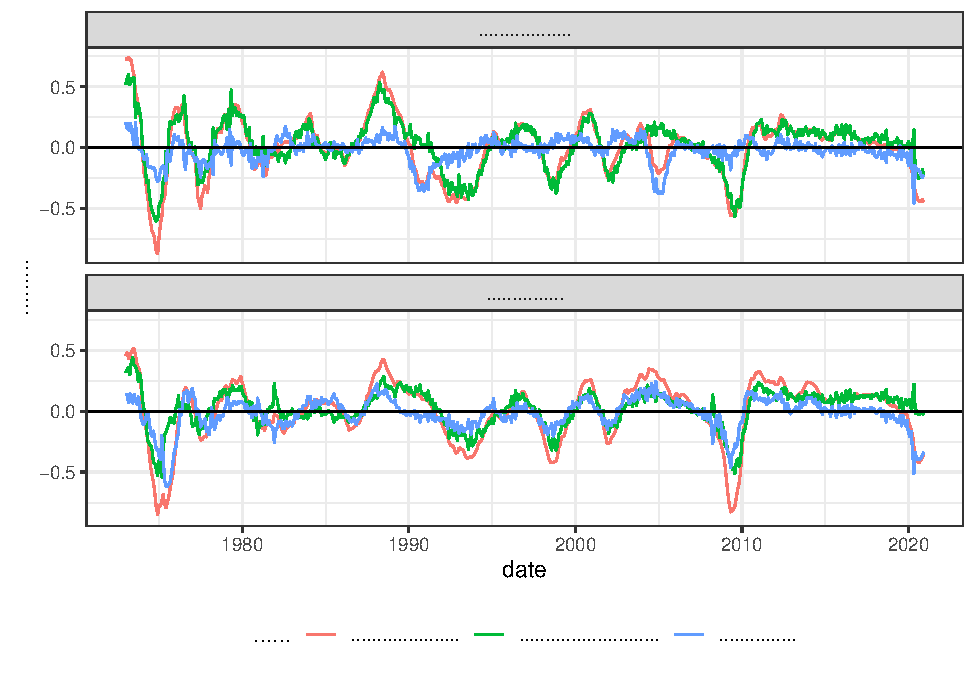
\includegraphics{test_files/figure-latex/unnamed-chunk-9-1.pdf}

\begin{itemize}
\tightlist
\item
  求人、求職への分解
\end{itemize}

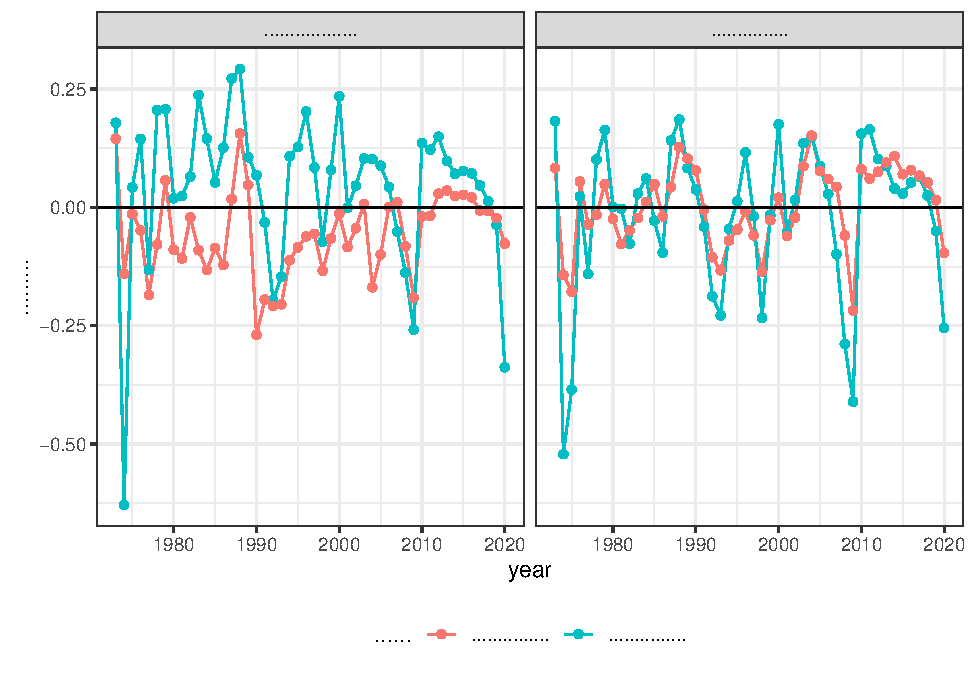
\includegraphics{test_files/figure-latex/unnamed-chunk-10-1.pdf}

\hypertarget{ux30dfux30b9ux30deux30c3ux30c1}{%
\chapter{ミスマッチ}\label{ux30dfux30b9ux30deux30c3ux30c1}}

\hypertarget{ux65b9ux6cd5-1}{%
\section{方法}\label{ux65b9ux6cd5-1}}

\begin{itemize}
\item
  Apply the mismatch index proposed by \citet{csahin2014mismatch}.
\item
  The mismatch index, \(M_t\), is defined as
\end{itemize}

\[M_t = \frac{h_t^{*}-h_t}{h_t},\]
where \(h_t\) and \(h_t^*\) are actual and counter-factual numbers of new employment, respectively.

\begin{itemize}
\item
  The counter-factual numbers is a solution of planner problem.
  The planner problem is to maximize the number of new employment, given the making function \(\mu_{jt}(u_{jt},v_{jt})\), the number of vacancy \(v_{jt}\), and the total number of job seeker \(u_{t}\).
\item
  Formally,
\end{itemize}

\[h_t^*=\max_{u_{jt}} \sum_j h_{jt},\]
subject to

\[h_{jt}=\mu_{jt}(u_{jt},v_{jt}),\ \ \ \ (matching\ function)\]
and

\[\sum_{j}u_{jt}=u_t.\ \ \ \ (Resource\ constrint)\]

\begin{itemize}
\tightlist
\item
  The estimation process is follows
\end{itemize}

\begin{enumerate}
\def\labelenumi{\arabic{enumi}.}
\tightlist
\item
  Suppose a parametric specification on the matching function as \(\mu_{jt}(u_{jt},v_{jt})=A_{jt}u_{jt}^{1-\beta}v_{jt}^{\beta}\), where \(A_{jt}=exp(f_t,f_j,\epsilon_{jt})\), \(f_t\) and \(f_j\) are time and sector fixed-effects, respectively.
  The parametric assumption obtains the closed solution of the planner problem;
\end{enumerate}

\[h_t^*=\max_{u_{jt}} \sum_j exp(f_t,f_j,\epsilon_{jt})\times v_{jt}^{\beta}\times (u_{jt}^*)^{1-\beta},\]
where
\[u_{jt}^*=\frac{A_{jt}^{1/\beta}v_{jt}}{\sum_{j'}A_{j't}^{1/\beta}v_{j't}}u_{t}.\ \ \ \ (optimal\ allocation)\]

\begin{enumerate}
\def\labelenumi{\arabic{enumi}.}
\setcounter{enumi}{1}
\tightlist
\item
  Estimate the log-transfer matching function
\end{enumerate}

\[\log(h_{jt}/u_{jt})=f_{j}+f_{t}+\beta\times\log(v_{jt}/u_{jt})+\epsilon_{jt}.\]

\begin{enumerate}
\def\labelenumi{\arabic{enumi}.}
\setcounter{enumi}{2}
\tightlist
\item
  Calculate the mismatch index with estimated parameters in Step 2.
\end{enumerate}

\hypertarget{aggregate-mismatch}{%
\section{Aggregate mismatch}\label{aggregate-mismatch}}

\begin{itemize}
\tightlist
\item
  Occupational mismatch by March, 2021.
\end{itemize}

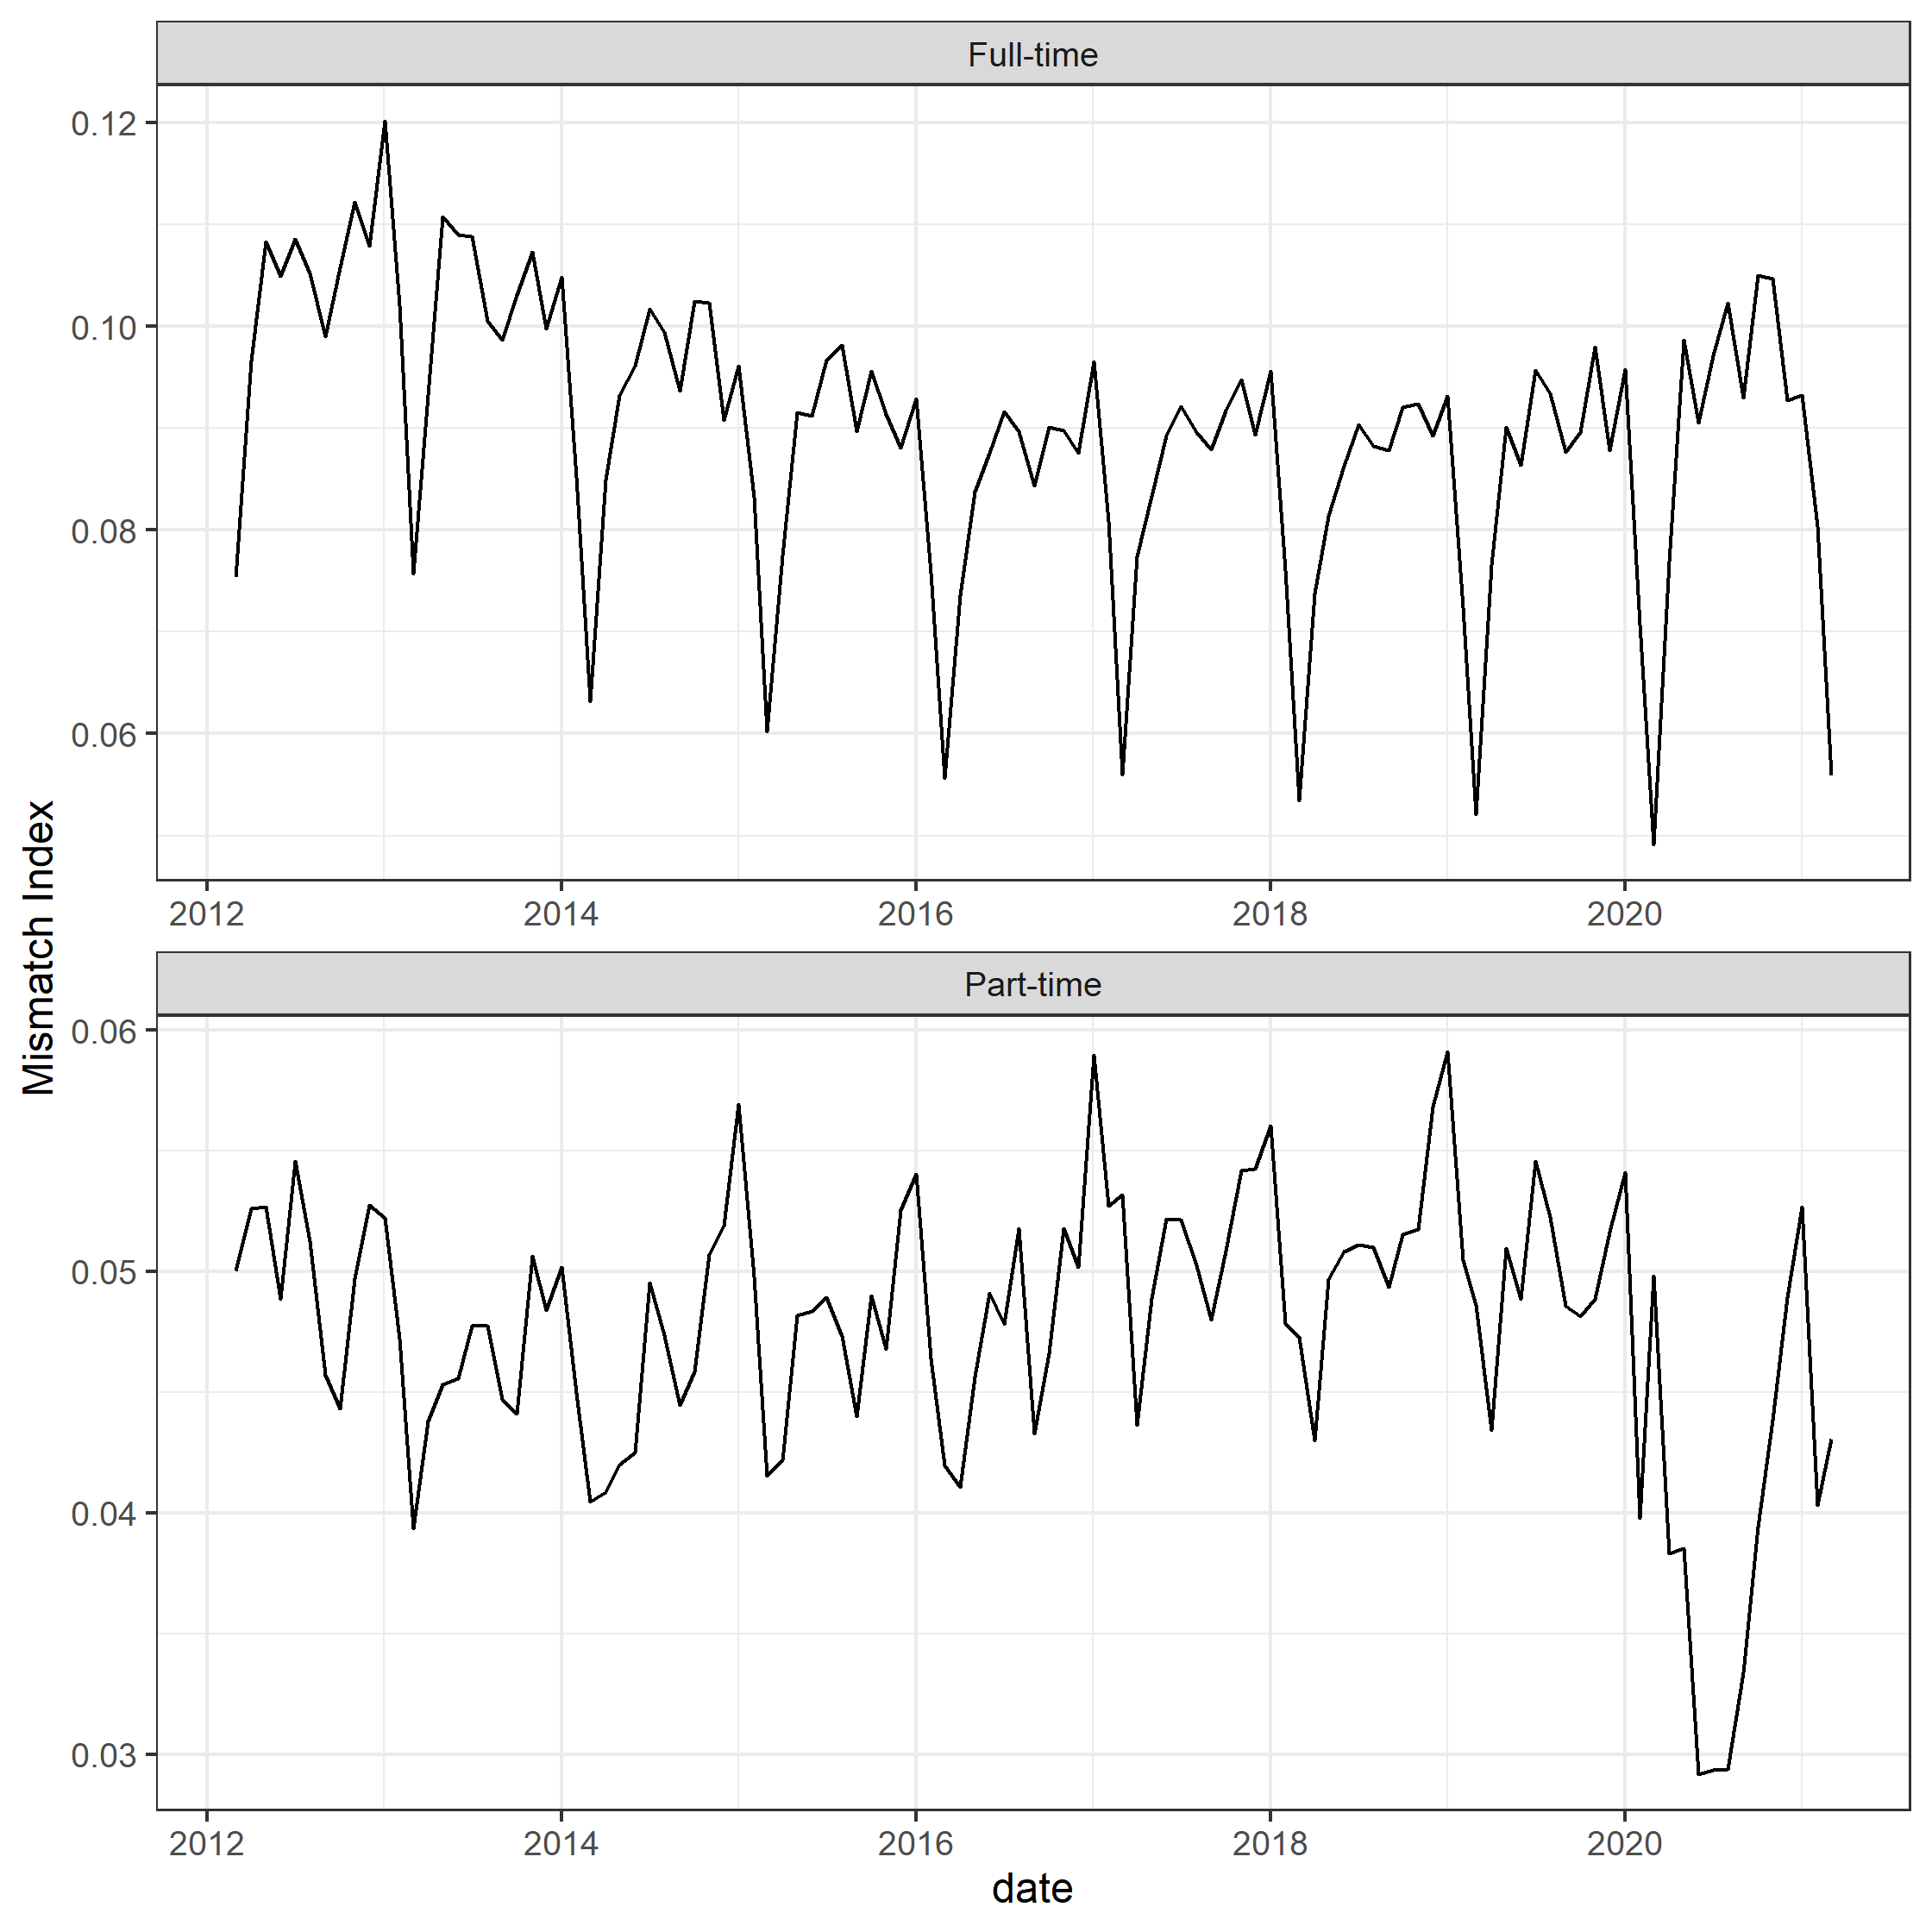
\includegraphics[width=31.11in]{R/figure/occ_mismatch}

  \bibliography{book.bib,packages.bib}

\end{document}
